\documentclass{article}
\usepackage{amsmath, tikz, enumerate, sfmath, bm, multicol, tcolorbox}
\renewcommand{\familydefault}{\sfdefault}
\usepackage[top = 0.5in, bottom = 0.5in, left = 1in, right = 1in]{geometry}
\pagestyle{empty}
\raggedright
\tikzset{>=stealth}
\usetikzlibrary{calc}
\begin{document}
\section*{Matrix Multiplication}

\begin{tcolorbox}[colframe=orange!70!white, coltitle=black, title=\textbf{Summary}]
\begin{enumerate}
    \item Matrix multiplication creates new basis vectors $\hat{\imath}$ and $\hat{\jmath}$.
    \item An $m \times n$ matrix can be multiplied by an $n \times r$ matrix to make an $m \times r$ matrix.
    \item Matrix multiplication transforms the coordinate plane itself as a series of compositions of functions.
\end{enumerate}
\end{tcolorbox}

\subsection*{Matrix Times a Vector}

Matrix multiplication does not work the way you might think. For instance, if 
\[ A = \begin{bmatrix} 3 & -2 \\ 1 & 0 \end{bmatrix} \quad \text{and} \quad B = \begin{bmatrix} -1 & 4 \\ 5 & 6 \end{bmatrix}
\]
\vspace{1in}

Then $AB$ is not $\begin{bmatrix} -3 & -8 \\ 5 & 0 \end{bmatrix}$. In other words, we don't multiply corresponding elements.	\vspace{1in}

In order to even multiply a matrix by a vector or another matrix, the number of columns in the first matrix \emph{must} equal the number of rows (for the vector or matrix) in the second.	\vspace{1in}

\newpage

Suppose we have the basis vector $\hat{\imath} = \begin{bmatrix} 1 \\ 0 \end{bmatrix}$. What happened to $\hat{\imath}$ when we multiply it by the matrix $\begin{bmatrix} 2 & 0 \\ 0 & 2 \end{bmatrix}$?
\bigskip

\[
\begin{bmatrix}
2 & 0 \\ 0 & 2 
\end{bmatrix}
\begin{bmatrix}
1 \\ 0
\end{bmatrix}
\]
\vfill

\begin{center}
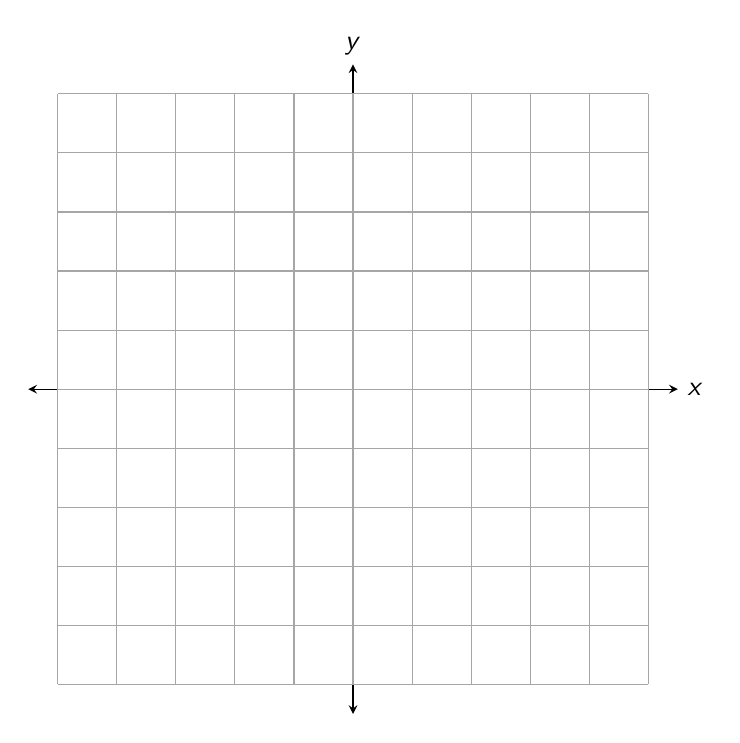
\begin{tikzpicture}[scale=0.75]
\draw[<->] (-5.5,0) -- (5.5,0) node [right] {$x$};
\draw[<->] (0,-5.5) -- (0,5.5) node [above] {$y$};
\draw[gray!70] (-5,-5) grid (5,5);
\end{tikzpicture}
\end{center}

\vfill


\newpage



{\color{red}\textbf{Example 1.}} What are the coordinates of $\hat{\jmath} = \begin{bmatrix} 0 \\ 1 \end{bmatrix}$ when you multiply it by 
$
\begin{bmatrix}
3 & 0 \\
0 & 3
\end{bmatrix}
$
\bigskip

\[
\begin{bmatrix}
3 & 0 \\
0 & 3
\end{bmatrix}
\begin{bmatrix} 0 \\ 1 \end{bmatrix}
\]

\vfill

\begin{center}
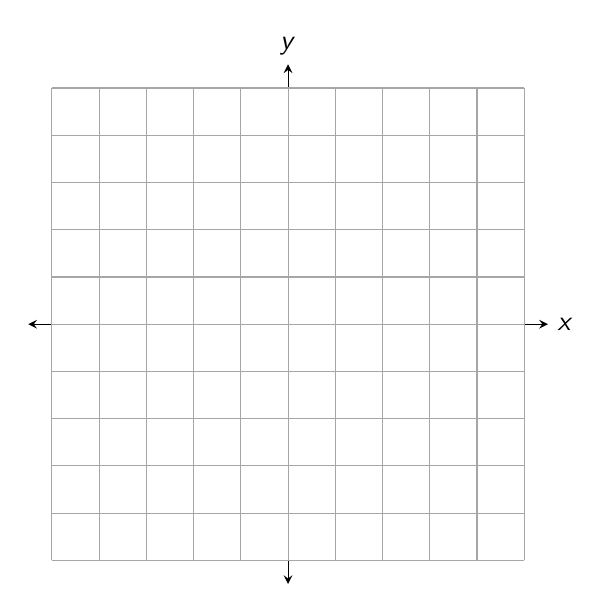
\begin{tikzpicture}[scale=0.6]
\draw[<->] (-5.5,0) -- (5.5,0) node [right] {$x$};
\draw[<->] (0,-5.5) -- (0,5.5) node [above] {$y$};
\draw[gray!70] (-5,-5) grid (5,5);
\end{tikzpicture}
\end{center}

\vfill

\newpage

Suppose we have the vector $\vec{v} = \begin{bmatrix} 2 \\ 1 \end{bmatrix}$. This can be written using the basis vectors $\hat{\imath}$ and $\hat{\jmath}$ as $\vec{v} = 2\hat{\imath} + 1\hat{\jmath}$.
\begin{center}
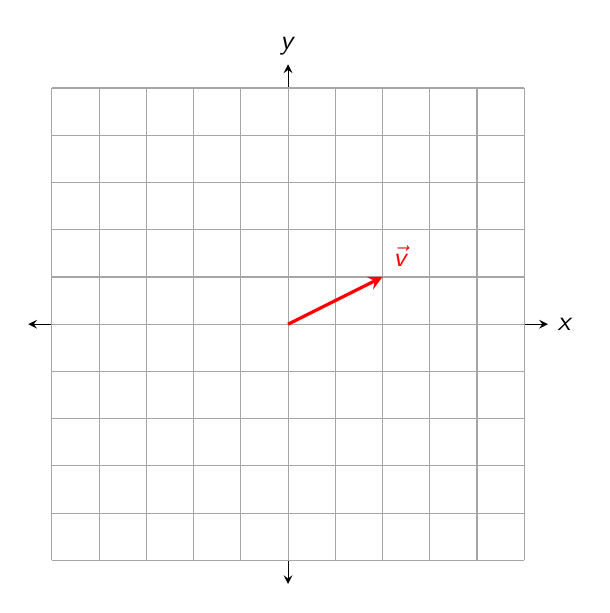
\begin{tikzpicture}[scale=0.6]
\draw[<->] (-5.5,0) -- (5.5,0) node [right] {$x$};
\draw[<->] (0,-5.5) -- (0,5.5) node [above] {$y$};
\draw[gray!70] (-5,-5) grid (5,5);
\draw[color=red, very thick, ->] (0,0) -- (2,1) node [above right] {$\vec{v}$};
\end{tikzpicture}
\end{center}

What happens when we multiply $\vec{v}$ by the matrix
$
\begin{bmatrix} 2 & 0 \\ 0 & 2 \end{bmatrix}
$
\bigskip

\[
\begin{bmatrix} 2 & 0 \\ 0 & 2 \end{bmatrix}
\begin{bmatrix} 2 \\ 1  \end{bmatrix}
\]

\vfill

\begin{center}
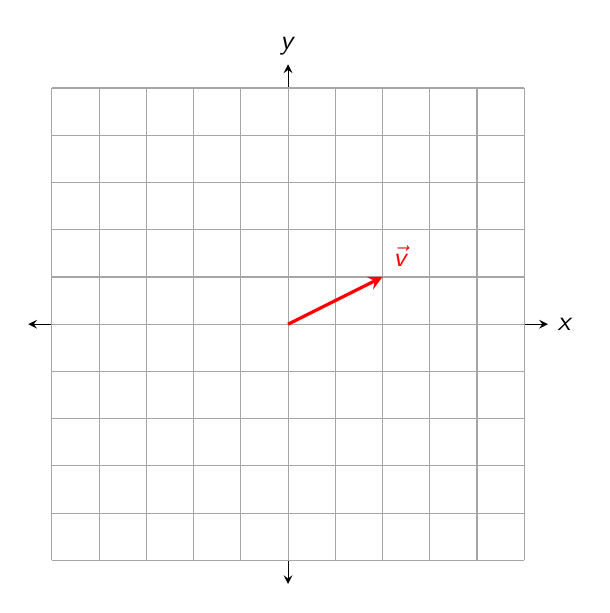
\begin{tikzpicture}[scale=0.6]
\draw[<->] (-5.5,0) -- (5.5,0) node [right] {$x$};
\draw[<->] (0,-5.5) -- (0,5.5) node [above] {$y$};
\draw[gray!70] (-5,-5) grid (5,5);
\draw[color=red, very thick, ->] (0,0) -- (2,1) node [above right] {$\vec{v}$};
\end{tikzpicture}
\end{center}

\newpage

{\color{red}\textbf{Example 2.}} Find the product and graph the result.
\[
\begin{bmatrix}
3 & -2 \\
1 & 1
\end{bmatrix}
\begin{bmatrix}
2 \\ 1
\end{bmatrix}
\]

\vfill

\begin{center}
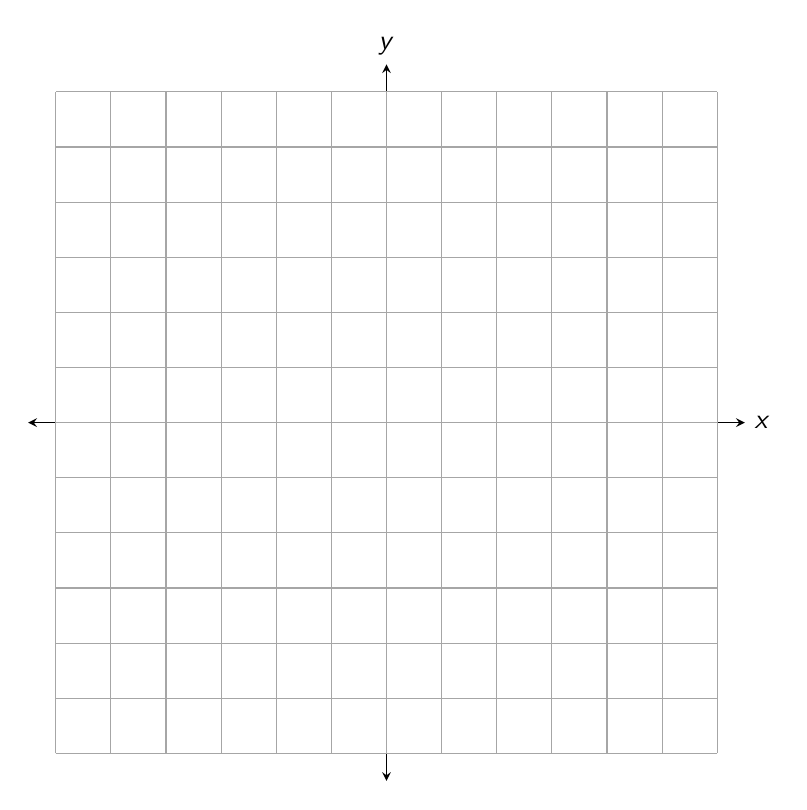
\begin{tikzpicture}[scale=0.7]
\draw[<->] (-6.5,0) -- (6.5,0) node [right] {$x$};
\draw[<->] (0,-6.5) -- (0,6.5) node [above] {$y$};
\draw[gray!70] (-6,-6) grid (6,6);
\end{tikzpicture}
\end{center}

\vspace{1in}

\newpage


\subsection*{Matrix Times a Matrix}

We can look at multiplying matrices as where $\hat{\imath}$ and $\hat{\jmath}$ end up in the coordinate plane. \newline\\

{\color{red}\textbf{Example 3.}} Explain the following problem visually 
\[
\begin{bmatrix}
0 & -1 \\
1 & 0
\end{bmatrix}
\begin{bmatrix}
1 & 0 \\
0 & 1
\end{bmatrix}
\]

\vfill

\begin{center}
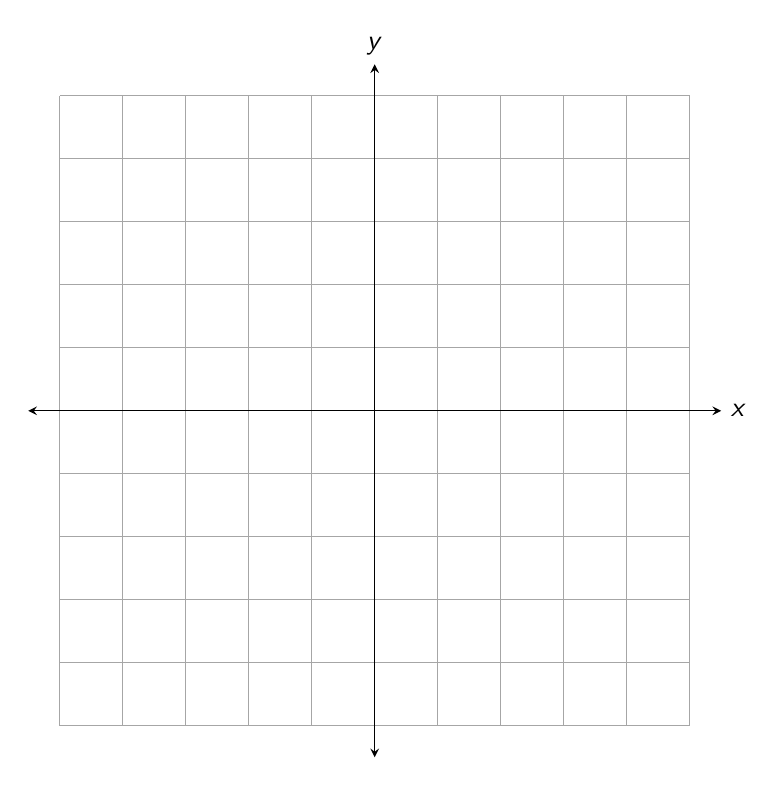
\begin{tikzpicture}[scale=0.8]
\draw [gray!70] (-5,-5) grid (5,5);
\draw[<->] (-5.5,0) -- (5.5,0) node [right] {$x$};
\draw[<->] (0,-5.5) -- (0,5.5) node [above] {$y$};
\end{tikzpicture}
\end{center}

\vspace{1in}

\newpage

{\color{red}\textbf{Example 4.}} Given $A = \begin{bmatrix} 1 & 0 \\ 0 & 1 \end{bmatrix}$, determine the effect of each product.

\begin{enumerate}[(a)]
	\item $\begin{bmatrix} 0 & -1 \\ 1 & 0 \end{bmatrix}  \begin{bmatrix} 1 & 0 \\ 0 & 1 \end{bmatrix}$.	\newline\\
	\begin{flushright}
	\begin{tikzpicture}
	\draw[gray!70] (-3,-3) grid (3,3);
	\draw[<->] (-3.5,0) -- (3.5,0) node [right] {$x$};
	\draw[<->] (0,-3.5) -- (0,3.5) node [above] {$y$};
	\end{tikzpicture}
	\end{flushright}
    \vfill
    
	\item $\begin{bmatrix} 1 & 0 \\ 1 & 1
 \end{bmatrix}  \begin{bmatrix} 1 & 0 \\ 0 & 1 \end{bmatrix}$  \label{ex4b} \newline\\
 
    \begin{flushright}
	\begin{tikzpicture}
	\draw[gray!70] (-3,-3) grid (3,3);
	\draw[<->] (-3.5,0) -- (3.5,0) node [right] {$x$};
	\draw[<->] (0,-3.5) -- (0,3.5) node [above] {$y$};
	\end{tikzpicture}
	\end{flushright}
\end{enumerate}

\newpage

In general, we can think of matrix multiplication like a composition of functions. \newline\\

Each multiplication leads to a new transformation of coordinates $\hat{\imath}$ and $\hat{\jmath}$:

\begin{itemize}
    \item Scaling $\hat{\imath}$ and/or $\hat{\jmath}$
    \item Rotating $\hat{\imath}$ and/or $\hat{\jmath}$
    \item Shearing $\hat{\imath}$ and/or $\hat{\jmath}$
    \item Changing the orientation of $\hat{\imath}$ and $\hat{\jmath}$
\end{itemize}

\vfill

For instance, in Example 4\ref{ex4b}, when we multiplied by the matrix   \newline\\ $\begin{bmatrix} 1 & 0 \\ 1 & 1 \end{bmatrix}$   \newline\\ it transformed the coordinate plane by shearing $\hat{\imath}$:   \newline\\

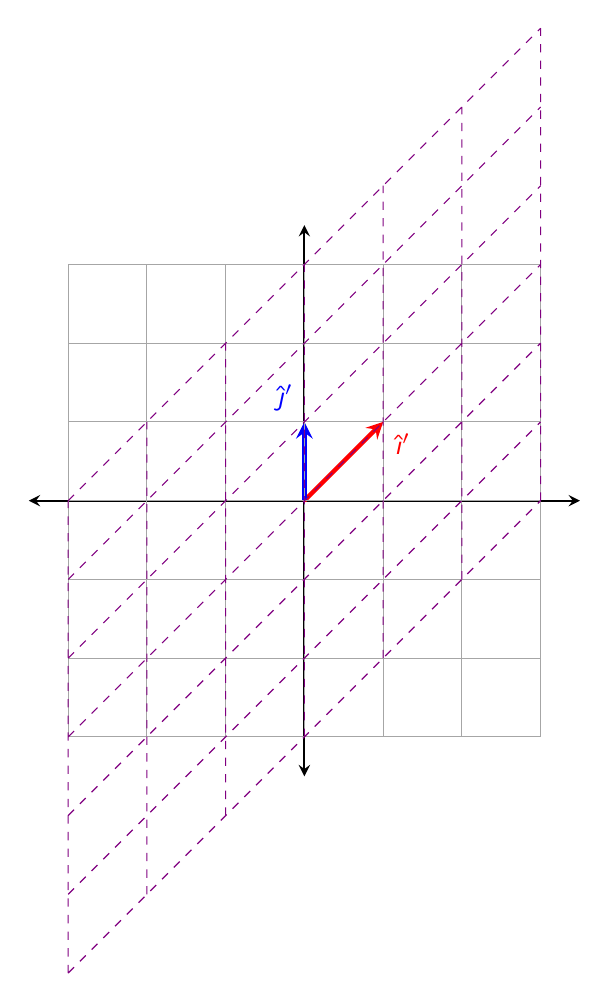
\begin{tikzpicture}
\draw[<->, thick] (-3.5,0) -- (3.5,0);
\draw[<->, thick] (0,-3.5) -- (0,3.5);
\draw[->, ultra thick, red] (0,0) -- (1,1) node [below right] {$\hat{\imath}'$};
\draw[->, ultra thick, blue] (0,0) -- (0,1) node [above left] {$\hat{\jmath}'$};
\draw [gray!70] (-3, -3) grid (3, 3);
\pgftransformcm{1}{1}{0}{1}{\pgfpoint{0cm}{0cm}}
\draw[dashed, violet] (-3,-3) grid (3,3);
\end{tikzpicture}

\newpage

{\color{red}\textbf{Example 5.}} Find each product.	
 
 \begin{enumerate}[(a)] 
 \item \quad $\begin{bmatrix} 2 & 1 \\ 1 & 2 \end{bmatrix} \begin{bmatrix} 1 &- 1 \\ 0 & 3 \end{bmatrix}$
 
    \begin{flushright}
	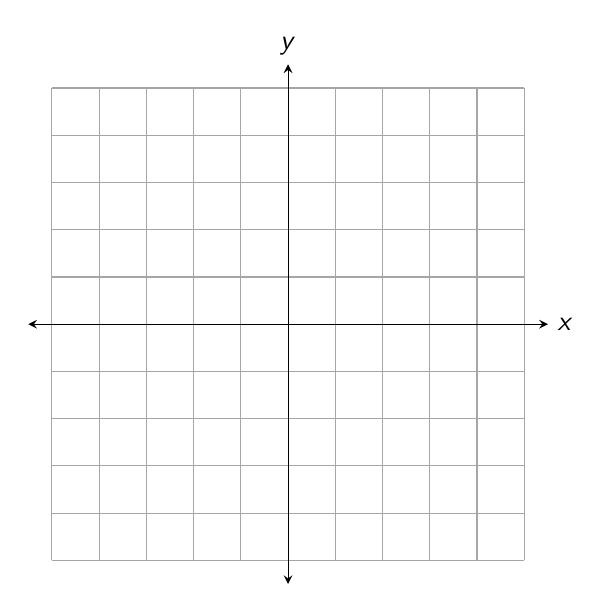
\begin{tikzpicture}[scale=0.6]
	\draw[gray!70] (-5,-5) grid (5,5);
	\draw[<->] (-5.5,0) -- (5.5,0) node [right] {$x$};
	\draw[<->] (0,-5.5) -- (0,5.5) node [above] {$y$};
	\end{tikzpicture}
	\end{flushright}
\vfill
 \item \quad $\begin{bmatrix} 1 &- 1 \\ 0 & 3 \end{bmatrix} \begin{bmatrix} 2 & 1 \\ 1 & 2 \end{bmatrix}$
 \begin{flushright}
	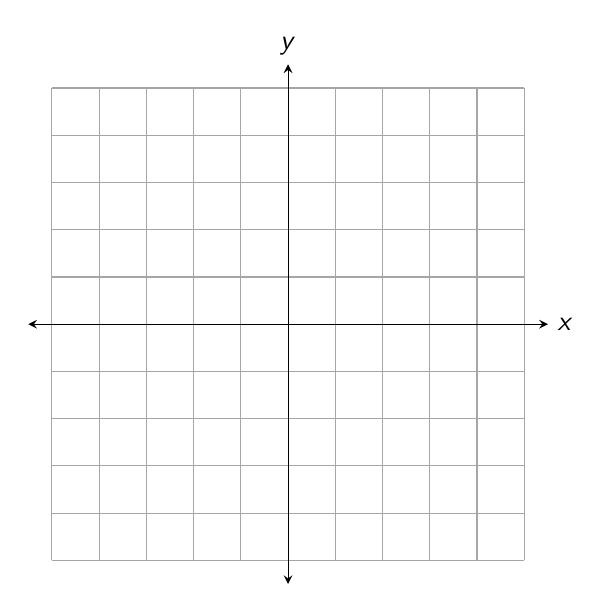
\begin{tikzpicture}[scale=0.6]
	\draw[gray!70] (-5,-5) grid (5,5);
	\draw[<->] (-5.5,0) -- (5.5,0) node [right] {$x$};
	\draw[<->] (0,-5.5) -- (0,5.5) node [above] {$y$};
	\end{tikzpicture}
	\end{flushright}
\end{enumerate}



\newpage

\begin{enumerate}[(a)] \addtocounter{enumi}{2}
 \item \quad $\begin{bmatrix} 2 & 4 \\ -2 & 3 \\ 5 & 1 \end{bmatrix}$ $\begin{bmatrix}
 -3 & 6 \\ 0 & -2 
 \end{bmatrix}$
 \vfill
 
 \item \quad $\begin{bmatrix}
 -3 & 6 \\ 0 & -2 
 \end{bmatrix}$ $\begin{bmatrix} 2 & 4 \\ -2 & 3 \\ 5 & 1 \end{bmatrix}$
 \vfill
\end{enumerate}

\newpage

\begin{enumerate}[(a)] \addtocounter{enumi}{4} 
\item \quad $\begin{bmatrix} 1 & -2 \end{bmatrix} \begin{bmatrix}
4 & -1 \\ 5 & 1 
\end{bmatrix}$
\vfill

\item \quad $\begin{bmatrix}
0 & 2 & -1 \\ 4 & 1 & 0 \\ 0 & -1 & 2
\end{bmatrix}$
$\begin{bmatrix}
4 & 3 & 0 \\ -1 & 0 & 2 \\ 1 & 0 & -2
\end{bmatrix}$
\end{enumerate}
\vfill

 
 
\end{document}
